%% Use \documentclass[print]{dissertation} to export the document
\documentclass[]{tesefop}

%%%%%%%%%%%%%%%%%%%%%%%%% Configuração: dados pessoais %%%%%%%%%%%%%%%%%%%%%%%%%
% FIXME Substituir 'Nome completo do aluno' pelo seu nome.
\newcommand{\autor}{Nome completo do aluno}
% FIXME Se for do sexo feminino, descomente a linha a seguir.
% \def\femaleAuthor{}

% FIXME Substituir 'Título da defesa' pelo título da defesa.
\newcommand{\titulo}{Título da defesa}
% FIXME Se estiver no programa de mestrado, descomente a linha a seguir.
% \def\mestrado{}
% FIXME Deixe descomente apenas a linha referente ao departamento.
% \def\matematica{}
\def\aplicada{}
% \def\estatistica{}

% FIXME Substituir 'Nome completo do orientador' pelo nome completo do seu
% orientador.
\newcommand{\orientador}{Nome completo do orientador}
% FIXME Se for orientado por uma mulher, descomente a linha a seguir.
% \def\femaleOrientador{}

% FIXME Substituir 'Nome completo do coorientador' pelo nome completo do seu
% coorientador. Caso não tenha coorientador, comente a linha a seguir.
\newcommand{\coorientador}{Nome completo do coorientador}
% FIXME Se for coorientado por uma mulher, descomente a linha a seguir.
% \def\femaleCoorientador{}

% FIXME Substituir 'Ano' pelo ano em que ocorreu sua defesa.
\newcommand{\ano}{Ano}




\begin{document}
	
	\thispagestyle{plain}
\noindent% just to prevent indentation narrowing the line width for this line
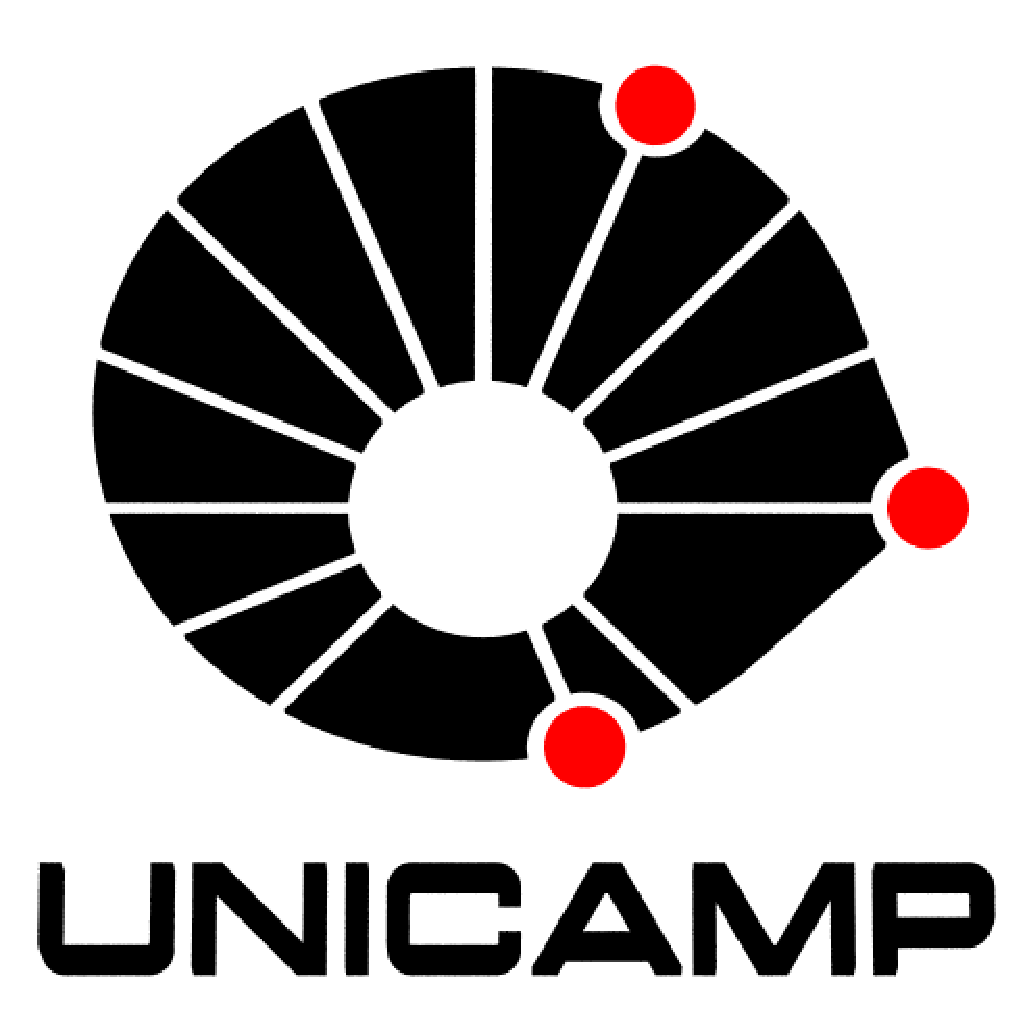
\includegraphics[width=0.10\textwidth]{imagens/logo-unicamp}%
\begin{minipage}[b]{0.7\textwidth}
	\centering
	\textbf{Universidade Estadual de Campinas} \\
\vspace{0.5cm}

\textbf{Faculdade de Odontologia de Piracicaba}
\end{minipage}%

\includegraphics[width=0.10\textwidth]{imagens/logo-fop}

\vspace{4cm}
\begin{center}
	% O tamanho da fonte deve ser 16pt.
	% Deve-se utilizar caixa alta.
	{\Large\textsc{\autor}}
\end{center}
\vspace{4cm}
\begin{center}
	% O tamanho da fonte deve ser 16pt em negrito.
	% Deve-se utilizar caixa alta.
	{\Large\textbf{\textsc{\titulo}}}
\end{center}
\vfill
\begin{center}
	% O tamanho da fonte deve ser 12pt em negrito.
	% Deve-se utilizar caixa alta.
	\textbf{Piracicaba \\ \ano}
\end{center}

	\thispagestyle{plain}


\begin{center}


\end{center}
\vfill
\begin{center}
  {\large\textbf{\textsc{\autor}}}
\end{center}
\vfill
\begin{center}
  {\Large\textbf{\textsc{\titulo}}}
\end{center}
\vfill

\begin{flushright}
  \begin{minipage}[c]{.5\textwidth}
    \ifx\mestrado\undefined
    Tese
    \else
    Dissertação
    \fi
    apresentada ao Instituto de Matemática,
    Estatística e Computação Científica da Universidade
    Estadual de Campinas como parte dos requisitos exigidos
    para a obtenção do título de
    \ifx\mestrado\undefined
    \ifx\femaleAuthor\undefined
    Doutor
    \else
    Doutora
    \fi
    \else
    \ifx\femaleAuthor\undefined
    Mestre
    \else
    Mestra
    \fi
    \fi
    em
    \ifx\matematica\undefined
    \else
    matemática.
    \fi
    \ifx\aplicada\undefined
    \else
    matemática aplicada.
    \fi
    \ifx\estatistica\undefined
    \else
    estatística.
    \fi
  \end{minipage}
\end{flushright}
\vspace{.5cm}

\noindent
\textbf{Orientador\ifx\femaleOrientador\undefined
\else
a\fi: \orientador
}
\vspace{.25cm}

\ifx\coorientador\undefined
\else
\noindent
\textbf{Coorientador\ifx\femaleCoorientador\undefined
\else
a\fi: \coorientador
}
\vspace{.5cm}
\fi

\noindent
\begin{minipage}[c]{.5\textwidth}
  {\footnotesize\textsc{Este exemplar corresponde à versão final da
  \ifx\mestrado\undefined
  tese
  \else
  dissertação
  \fi
  defendida
  \ifx\femaleAuthor\undefined
  pelo aluno
  \else
  pela aluna
  \fi
  \autor,
  e orientada pel\ifx\femaleOrientador\undefined
  o\else
  a\fi{} Prof\ifx\femaleOrientador\undefined
  \else
  a\fi. Dr\ifx\femaleOrientador\undefined
  \else
  a\fi. \orientador.
  }}
\end{minipage}
\vspace{1cm}

\noindent
{\small\textbf{Assinatura
\ifx\femaleOrientador\undefined
do Orientador
\else
da Orientadora
\fi
}

\vspace{.5cm}
\noindent
\rule[1pt]{7cm}{.5pt}  % Linha para assinatura do orientador
}
\vspace{.5cm}

\ifx\coorientador\undefined
\else
\noindent
{\small\textbf{Assinatura
\ifx\femaleCoorientador\undefined
do Coorientador
\else
da Coorientadora
\fi
}

\vspace{.5cm}
\noindent
\rule[1pt]{7cm}{.5pt}  % Linha para assinatura do coorientador
}
\fi
\vfill
\begin{center}
  {\small\textbf{\textsc{ Campinas \\ \ano}}}
\end{center}

	\include{ficha_catalografica}
	\include{ficha_aprovacao}
	\section{Dedicatoria}



\blindtext %apague completamente esta linha.

	\section{Agradecimentos}

\blindtext %apague completamente esta linha.
	\include{listas}
	\section{Resumo}
	\section{Abstract}

\Blindtext %apague completamente esta linha.
	\section{Outro abstract}
	\section{Sumario}
	
	
	\tableofcontents
	
	\include{capitulo1/capitulo1}
    \include{capitulo2/capitulo2}
	\include{capitulo3/capitulo3}
	\include{capitulo4/capitulo4}
				
	
	

\end{document}